\documentclass{article}

\usepackage{graphicx}
\usepackage{tikz}
\usepackage{tikzsymbols}
\usetikzlibrary{calc,patterns,shapes.geometric}
\pagestyle{empty}
\usepackage[margin=0pt]{geometry}
\geometry{papersize={14in,12in}}

\def\centerarc[#1](#2)(#3:#4:#5){\draw[#1] ($(#2)+({#5*cos(#3)},{#5*sin(#3)})$) arc (#3:#4:#5);}

\begin{document}
	\begin{figure}
		\centering
		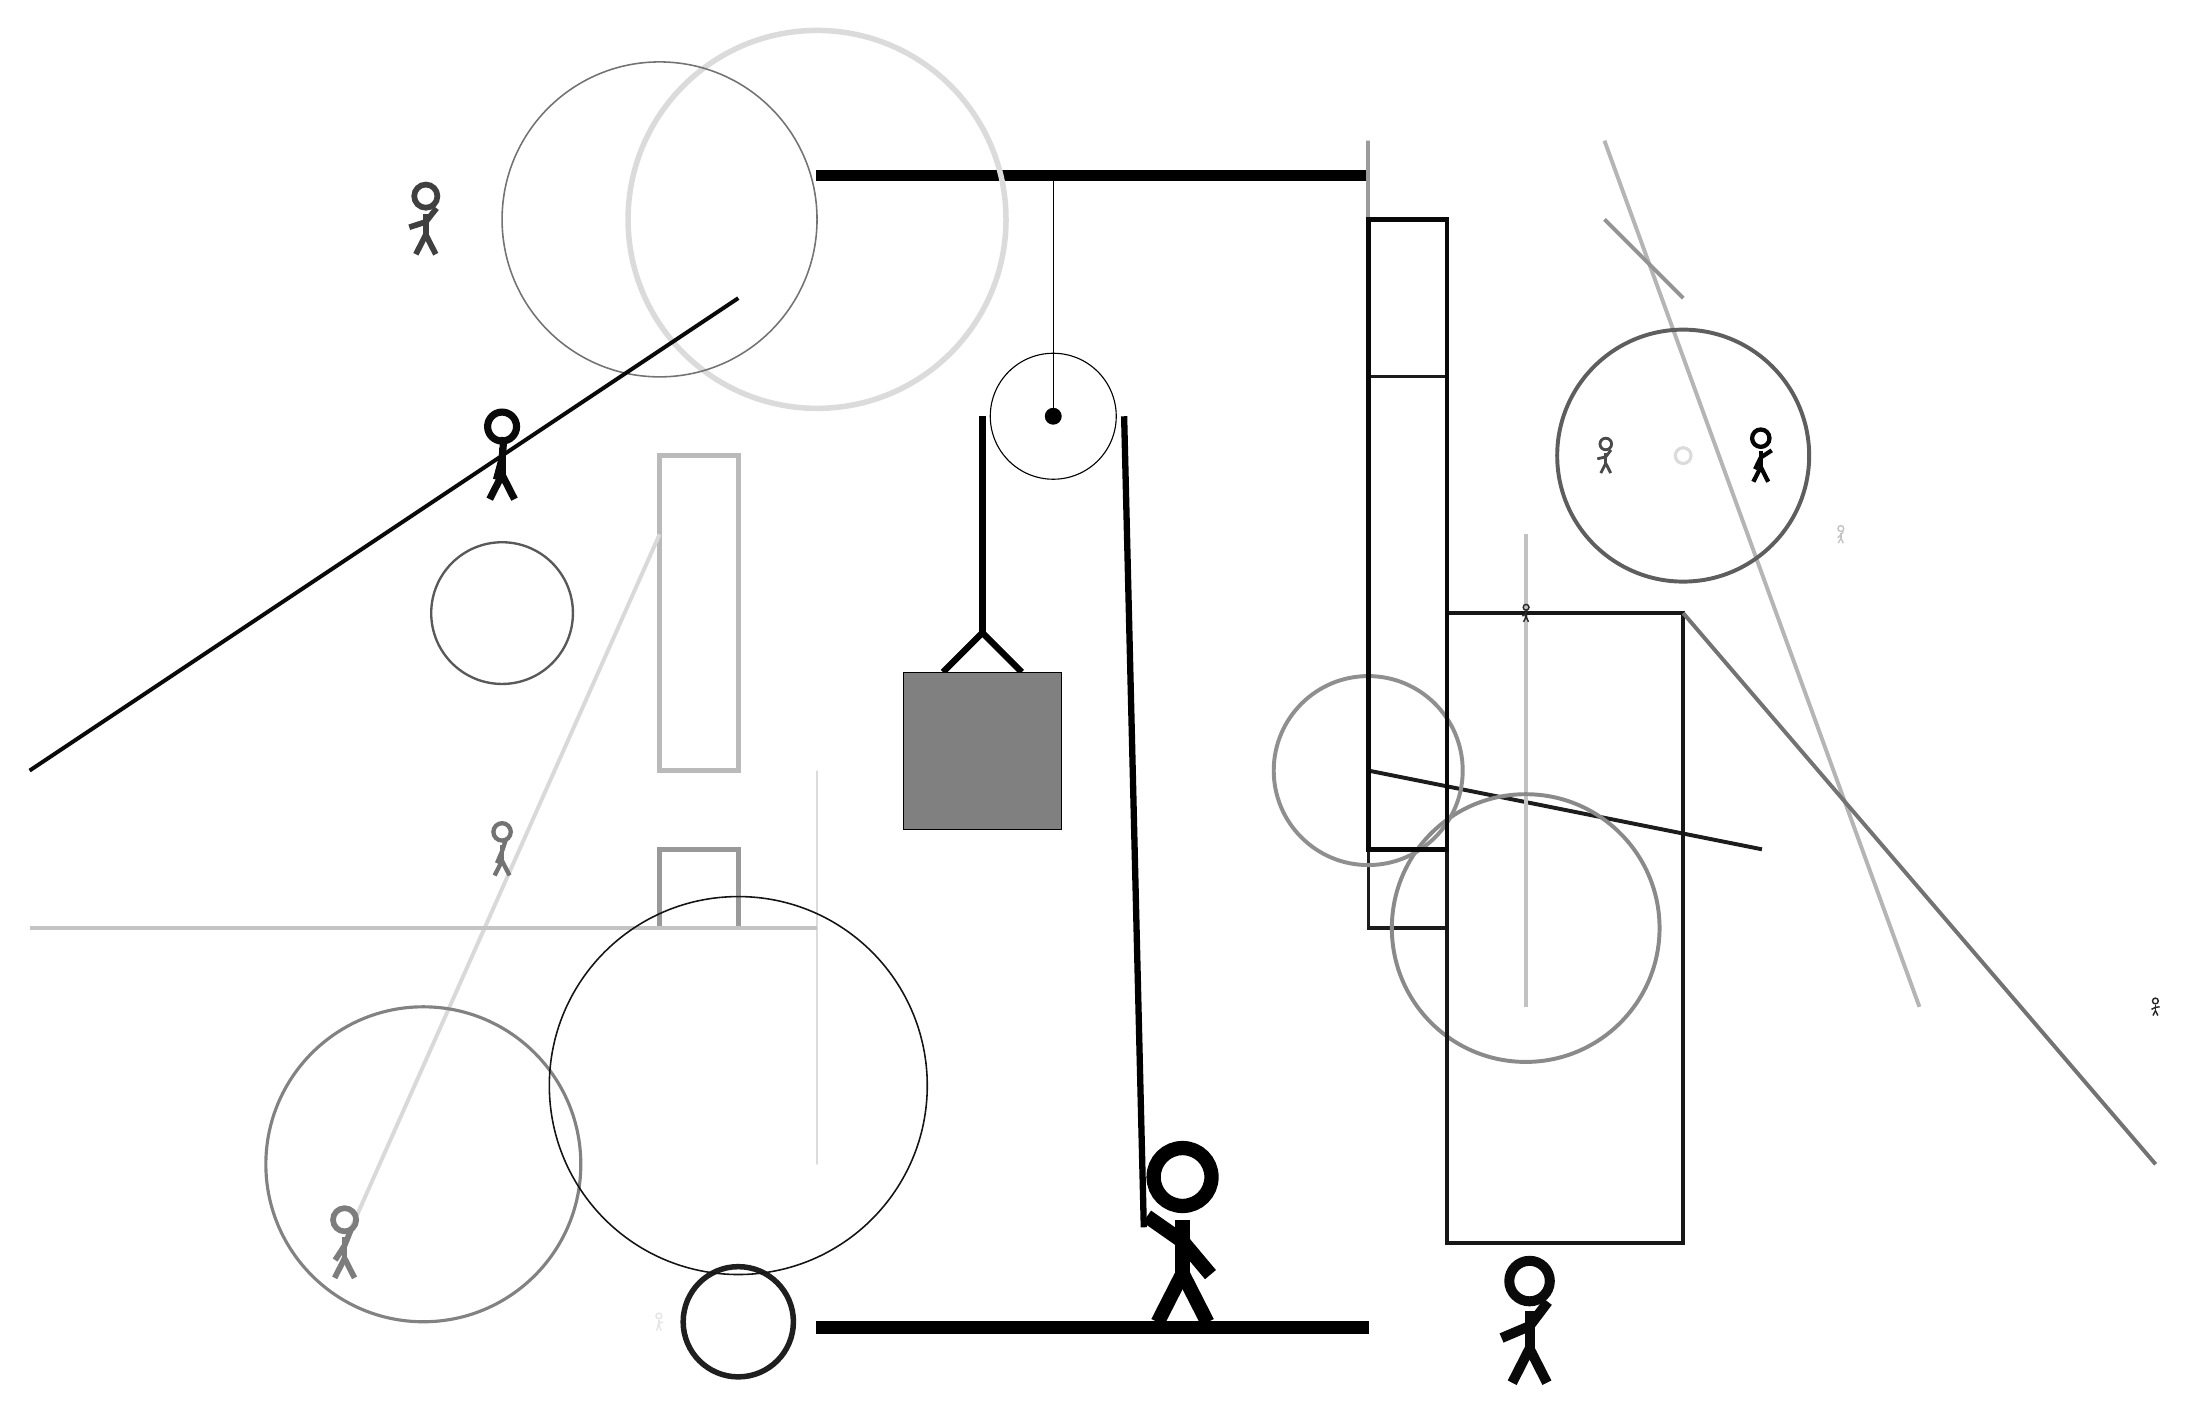
\begin{tikzpicture}
			%%%%% START %%%%%
			
			\draw[fill=black] (-2, 11.5) rectangle (5, 11.625);
			
			\draw (1, 8.5) circle (0.8);
			\draw[fill=black] (1, 8.5) circle (0.1);
			\draw (1, 11.5) -- (1, 8.5);
			
			\draw[line width=0.8mm] (-0.4, 5.25) -- (0.1, 5.75) -- (0.6, 5.25);
			\draw[fill=black!50] (-0.9, 5.25) rectangle (1.1, 3.25);
			
			\draw[line width=0.6mm, color=black!27] (-3, 4) rectangle (-4, 8);
			
			\draw[line width=0.3mm, color=black!14] (-2, 4) rectangle (-2, -1);
			\node[line width=0.2mm, color=black!96] at (7, -3) {\Strichmaxerl[7][23][53]};
			\node[line width=0.6mm, color=black!98] at (10, 8) {\Strichmaxerl[3][64][33]};
			\draw[line width=0.5mm, color=black!15](-4, 7) -- (-8, -2);
			\draw[line width=0.5mm, color=black!39] (5, 11) rectangle (5, 12);
			
			\draw[line width=0.5mm, color=black!89](10, 3) -- (5, 4);
			\draw[line width=0.5mm, color=black!24](7, 1) -- (7, 7);
			\node[line width=0.2mm, color=black!96] at (-6, 8) {\Strichmaxerl[5][75][85]};
			\node[line width=0.2mm, color=black!23] at (11, 7) {\Strichmaxerl[1][41][55]};
			
			\draw[line width=0.6mm, color=black!40] (-3, 2) rectangle (-4, 3);
			
			\draw [line width=0.7mm, color=black!14](-2, 11) circle (2.4);
			\draw[line width=0.4mm, color=black!89] (5, 2) rectangle (6, 9);
			
			\draw [line width=0.5mm, color=black!46](7, 2) circle (1.7);
			\node[line width=0.3mm, color=black!75] at (-7, 11) {\Strichmaxerl[4][18][52]};
			\draw[line width=0.5mm, color=black!29](8, 12) -- (12, 1);
			\draw [line width=0.5mm, color=black!44](5, 4) circle (1.2);
			\draw[line width=0.5mm, color=black!91] (6, 6) rectangle (9, -2);
			\node[line width=0.6mm, color=black!85] at (15, 1) {\Strichmaxerl[1][27][9]};
			\node[line width=0.2mm, color=black!51] at (-8, -2) {\Strichmaxerl[4][57][68]};
			\draw [line width=0.3mm, color=black!65](-6, 6) circle (0.9);
			
			\draw[line width=0.5mm, color=black!55](9, 6) -- (15, -1);
			\draw[line width=0.5mm, color=black!23](-2, 2) -- (-12, 2);
			\draw [line width=0.5mm, color=black!63](9, 8) circle (1.6);
			\draw [line width=0.4mm, color=black!49](-7, -1) circle (2.0);
			\draw [line width=0.4mm, color=black!14](9, 8) circle (0.1);
			\draw[line width=0.5mm, color=black!42](9, 10) -- (8, 11);
			\node[line width=0.2mm, color=black!84] at (7, 6) {\Strichmaxerl[1][32][81]};
			\draw [line width=0.2mm, color=black!55](-4, 11) circle (2.0);
			\draw[line width=0.6mm, color=black!97] (6, 3) rectangle (5, 11);
			\draw [line width=0.7mm, color=black!88](-3, -3) circle (0.7);
			
			\draw[line width=0.5mm, color=black!96](-3, 10) -- (-12, 4);
			\node[line width=0.3mm, color=black!71] at (8, 8) {\Strichmaxerl[2][13][53]};
			\node[line width=0.7mm, color=black!55] at (-6, 3) {\Strichmaxerl[3][67][72]};
			
			\draw [line width=0.2mm, color=black!92](-3, 0) circle (2.4);
			\node[line width=0.4mm, color=black!10] at (-4, -3) {\Strichmaxerl[1][74][2]};
			
			
			\draw[line width=0.8mm] (0.1, 8.5) -- (0.1, 5.75);
			\centerarc[line width=0.8mm](1, 8.5)(0:180:0.9);
			\draw[line width=0.8mm](1.9, 8.5) -- (2.15, -1.8);
			
			\node at (2.6, -1.9) {\Strichmaxerl[10][-35][-50]};
			
			\draw[fill=black] (-2, -3) rectangle (5, -3.15);
			
			%%%%% END %%%%%
		\end{tikzpicture}
	\end{figure}	
\end{document}